\section{Karnaugh maps}

\subsection{Two input K-maps}
\begin{Karnaughquatre}
  \phminterms{0,1,2,3}
\end{Karnaughquatre}

% \begin{example}
%   Convert the following truth table into a K-map.
% 
%   \noindent
%   \begin{tabular}{ll|l}
%     \toprule
%      A & B & f \\
%     \midrule
%     0 & 0 & 0 \\ 
%     0 & 1 & 1 \\ 
%     1 & 0 & 1 \\ 
%     1 & 1 & 0 \\ 
%     \bottomrule
%   \end{tabular}
% \end{example}
% \vspace{10em}

% \begin{prob}
%   Convert the following Venn Diagram into a K-map.
% 
%   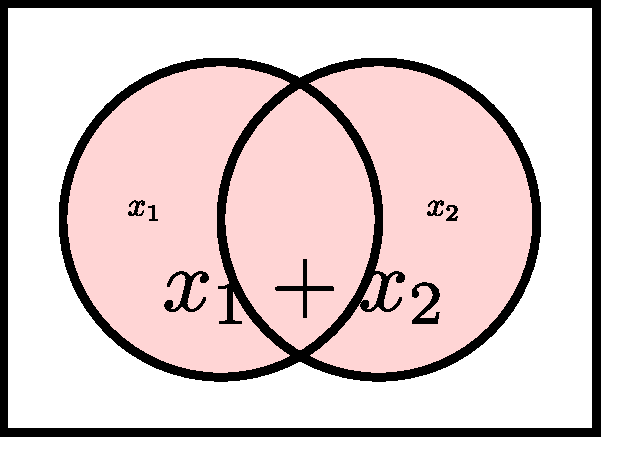
\includegraphics[width=0.2\linewidth]{OR_Venn.pdf}
% \end{prob}
% \vspace{10em}
  
\subsection{Three input K-maps}

\begin{Karnaughvuit}
  \phminterms{0,1,2,3,4,5,6,7}
\end{Karnaughvuit}

% \begin{prob}
%   Draw a K-map for the function $f = \bar{A}\bar{B}C + AB\bar{C}$.
% \end{prob}
% \vspace{10em}

\subsection{Four input K-maps}
\begin{Karnaugh}{AB}{CD}
  \phminterms{0,1,2,3,4,5,6,7,8,9,10,11,12,13,14,15}
\end{Karnaugh}


% \begin{prob}
%   Draw a K-map for a 4-input function $f = m_1 + m_2 + m_7 $.
% \end{prob}
% \vspace{10em}

\subsection{Five input K-maps}

A = 0
\begin{Karnaugh}{BC}{DE}
  \phminterms{0,1,2,3,4,5,6,7,8,9,10,11,12,13,14,15}
\end{Karnaugh} \hfill
A = 1
\begin{Karnaugh}{BC}{DE}
  \phmintermssixt{0,1,2,3,4,5,6,7,8,9,10,11,12,13,14,15}
\end{Karnaugh}

% \begin{prob}
%   Draw a K-map for a 5-input function $f = M_1 M_2 M_7 $.
% \end{prob}
% \vspace{10em}
\section{More Gates and notations summary}
\rotatebox[origin=c]{90}{
\begin{tabular}{lccp{0.2\linewidth}cp{0.2\linewidth}}
  \toprule
  Name & C/Verilog & Boolean expr. & Truth Table & (ANSI) symbol & K-map \\
  \midrule
  NAND Gate &
  \texttt{Q = \~{}(x1 \& x2)} &
  $Q = \overline{x_1 \cdot x_2} = \overline{x_1 x_2}$ &
 \mbox{\begin{tabular}{cc|c}
 \toprule
 $x_1$ & $x_2$ & $\overline{x_1 \cdot x_2}$ \\
 \midrule
 0 & 0 & 1 \\
 0 & 1 & 1 \\
 1 & 0 & 1 \\
 1 & 1 & 0 \\
 \bottomrule
 \end{tabular}} &
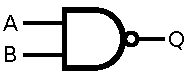
\includegraphics[width=0.2\linewidth]{NAND_ANSI_Labelled.pdf} &
\begin{minipage}[b][][t]{\linewidth}
\begin{Karnaughquatre}
\minterms{0,1,2}
\maxterms{3}
\end{Karnaughquatre}
\end{minipage}
\\
  NOR Gate &
\texttt{Q = \~{}(x1 | x2)} &
$Q = \overline{x_1 + x_2}$ &
\mbox{\begin{tabular}{cc|c}
  \toprule
  $x_1$ & $x_2$ & $\overline{x_1 + x_2}$ \\
  \midrule
  0 & 0 & 1 \\
  0 & 1 & 0 \\
  1 & 0 & 0 \\
  1 & 1 & 0 \\
  \bottomrule
\end{tabular}} &
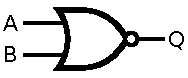
\includegraphics[width=0.2\linewidth]{NOR_ANSI_Labelled.pdf} & 
                                                               \begin{minipage}[b][][t]{\linewidth}
\begin{Karnaughquatre}
\minterms{3}
\maxterms{0,1,2}
\end{Karnaughquatre}
\end{minipage}
\\
XOR Gate &
\texttt{Q = x1 \^{} x2}
&
$ Q = x_1 \oplus x_2$
&
\mbox{\begin{tabular}{cc|c}
\toprule
$x_1$ & $x_2$ & $x_1 \oplus x_2$ \\
\midrule
0 & 0 & 0 \\
0 & 1 & 1 \\
1 & 0 & 1 \\
1 & 1 & 0 \\
\bottomrule
        \end{tabular}}
&
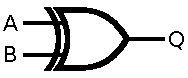
\includegraphics[width=0.2\linewidth]{XOR_ANSI_Labelled.pdf} &
\begin{minipage}[b][][t]{\linewidth}
\begin{Karnaughquatre}
\minterms{1,2}
\maxterms{0,3}
\end{Karnaughquatre}
\end{minipage}
\\
XNOR Gate &
\texttt{Q = \~{}(x1 \^{} x2)}
&
$ Q = \overline{x_1 \oplus x_2}$
&
\mbox{\begin{tabular}{cc|c}
        \toprule
        $x_1$ & $x_2$ & $\overline{x_1 \oplus x_2}$ \\
        \midrule
        0 & 0 & 1 \\
        0 & 1 & 0 \\
        1 & 0 & 0 \\
        1 & 1 & 1 \\
        \bottomrule
      \end{tabular}}
    &
    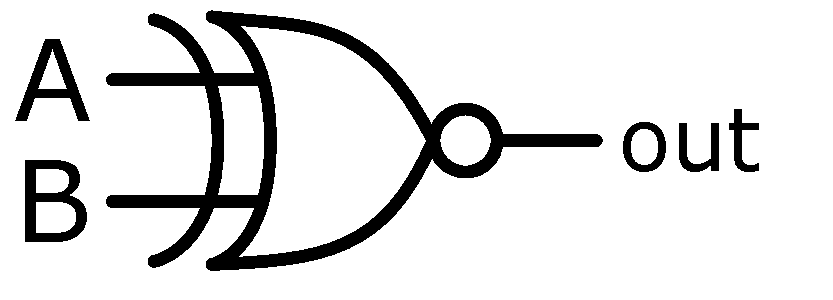
\includegraphics[width=0.2\linewidth]{XNOR_ANSI_Labelled.pdf} &
    \begin{minipage}[b][][t]{\linewidth}
      \begin{Karnaughquatre}
        \minterms{0,3}
        \maxterms{1,2}
      \end{Karnaughquatre}
    \end{minipage}
  \end{tabular}
}
\newpage


\begin{example}
  Convert the following Boolean expression into a K-map.
  $ f = \overline{A\bB + C}D $
\end{example}
\vspace{20em}

\begin{prob}
  Convert the following logic circuit into a K-map.\\
  \begin{tikzpicture}[circuit logic US]
    \matrix[column sep=7mm]{
      \node (A) {$A$}; & &  \node [or gate] (andAB) {}; & & & \\
      \node (B) {$B$}; & \node [not gate] (nB) {};  &  & \node [and gate] (orGC) {}; &  & \\
      \node (C) {$C$}; & & \node (C2) {}; & & & \node [and gate] (andHD) {}; \\
      \node (D) {$D$}; & &  & & \node (D2) {}; &\\
    };
    \draw (A) -- ++(right:3mm) |- (andAB.input 1);
    \draw (B) -- (nB.input);
    \draw (nB.output) -- ++(right:3mm) |- (andAB.input 2);

    \draw (andAB.output) to [edge label=g] ++(right:3mm) |- (orGC.input 1);
    \draw (C) -- (C2.east) -- ++(right:3mm) |- (orGC.input 2);

    % \draw (orGC.output)  to [edge label=h] (andHD.input);

    \draw (orGC.output) to [edge label=h] ++(right:3mm) |- (andHD.input 1);
    \draw (D) -- (D2.east) -- ++(right:3mm) |- (andHD.input 2);
    
    \draw (andHD.output) to [edge label=f] ++(right:3mm);
  \end{tikzpicture}
\end{prob}
\vspace{20em}

\section{Boolean Algebra}

\subsection{Axioms of Boolean algebra}

\begin{enumerate}
\item 
  $ 0 \cdot 0 = 0 $
\item 
    $ 1 + 1 = 1 $
\item
    $ 1 \cdot 1 = 1 $
\item
    $ 0 + 0 = 0 $
\item
    $ 0 \cdot 1 = 1 \cdot 0 = 0 $
\item
      $ \bar{0} = 1 $
\item
        $ \bar{1} = 0 $
\item
      $ x = 0 \text{ if } x \ne 1$ 
    \item
      $ x = 1 \text{ if } x \ne 0$ 
\end{enumerate}

\subsection{Single variable theorems (Prove by drawing K-maps)}

\begin{enumerate}
\item $ x \cdot 0 = 0 $
  \vspace{5em}
\item $ x + 1 = 1 $
  \vspace{5em}
\item $ x \cdot 1 = x $
  \vspace{5em}
\item $ x + 0 = x $
  \vspace{5em}
\item $ x \cdot x = x $
  \vspace{5em}
\item $ x + x = x $
  \vspace{5em}
\item $ x \cdot \bar{x} = 0 $
  \vspace{5em}
\item $ x + \bar{x} = 1 $
  \vspace{5em}
\item $\bar{\bar{x}} = x $
  \vspace{5em}
\end{enumerate}

\begin{remark}[Duality]
  Swap $+$ with $\cdot$ and 0 with 1 to get another theorem
\end{remark}

\subsection{Two and three variable properties (Prove by K-maps)}

\begin{enumerate}
\item Commutative: $x\cdot y = y \cdot x$ , $x + y = y + x$
  \vspace{10em}
\item Associative: $x\cdot(y\cdot z) = (x \cdot y) \cdot z$, $x+(y+ z) = (x + y) + z$
  \vspace{10em}
\item Distributive: $x\cdot(y + z) = x \cdot y + x \cdot z$, $x + y \cdot z = (x + y) \cdot (y + z)$
  \vspace{10em}
\item Absorption: $x + x\cdot y = x$, $x \cdot (x+y) = x$
  \vspace{10em}
\item Combining: $x \cdot y + x \cdot \bar{y}$, $(x+y) \cdot (x + \bar{y}) = x$
  \vspace{10em}
\item DeMorgan's theorem: $\overline{x \cdot y} = \bar{x} + \bar{y}$,
  $\overline{x + y} = \bar{x} \cdot \bar{y}$.
  \vspace{10em}
\item Concensus:
  \begin{enumerate}
  \item $x + \bar{x}\cdot y = x + y$
    \vspace{10em}
  \item $x \cdot (\bar{x} + y) = x \cdot y$
    \vspace{10em}
  \item $x \cdot y + y\cdot z + \bar{x} \cdot z = x\cdot y + \bar{x} \cdot z$
    \vspace{10em}
  \item $(x + y) \cdot (y+ z) \cdot (\bar{x} + z) = (x+ y) \cdot (\bar{x} + z)$
    \vspace{10em}
  \end{enumerate}
\end{enumerate}

\begin{example}[Multiplexer]
  Multiplexer is a circuit used to select one of the input lines $x_1$ and $x_2$
  based only select input $s$. When $s=0$, $x_1$ is selected, $x_2$ is selected otherwise.
  Find a boolean expression and a circuit for multiplexer\\
  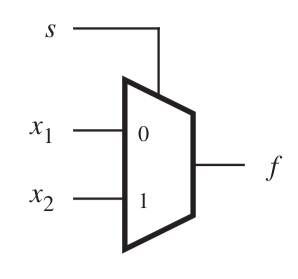
\includegraphics[width=0.2\linewidth]{multiplexer-symbol.png}
  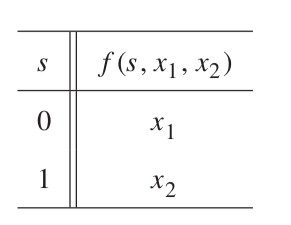
\includegraphics[width=0.2\linewidth]{multiplexer-spec.png}
\end{example}
\vspace{10em}

\begin{example}
  Simplify $f = \bA\bB\bC + A \bB\bC + A\bB\bC $ using boolean algebra.
\end{example}
\vspace{10em}

\begin{example}
  Simplify $f = \bA\bA\bC + \bA\bB C $ using K-maps.
\end{example}
\vspace{10em}